\chapter{Advanced Topics}\label{advanced}

We have covered a lot of material in the previous chapters,
but have only scratched the surface of what R can do \st{to} for us.
To wrap up,
we will look briefly at a few of its more advanced capabilities.

\section{How can we use Python with R?}

We can put Python code in R~Markdown documents:

\begin{lstlisting}
print("Hello R")
\end{lstlisting}

\begin{lstlisting}
Hello R
\end{lstlisting}

\noindent
but how can those chunks interact with our R and vice versa?
The answer is a package called \texttt{reticulate}
that provides two-way communication between Python and R.

By default,
\texttt{reticulate} uses the default version of Python on our computer:

\begin{lstlisting}
Sys.which("python")
\end{lstlisting}

\begin{lstlisting}
                 python 
"/anaconda3/bin/python" 
\end{lstlisting}

but we can configure it to use different versions,
or to use \texttt{virtualenv} or a \texttt{conda} environment.
\href{https://rstudio.github.io/reticulate/articles/versions.html}{The documentation}
has all of the details;
the short version is:

\begin{enumerate}
\item
  Run \texttt{install.packages("reticulate")} to install the package.
\item
  Set the environment variable \texttt{RETICULATE\_PYTHON}
  to point at the version of Python you want to use.
  This is necessary because you may have a system-installed version somewhere like \texttt{/usr/bin/python}
  and another version managed by \texttt{conda} somewhere else.
\item
  Close and relaunch RStudio.
\end{enumerate}

\begin{figure}[h]
  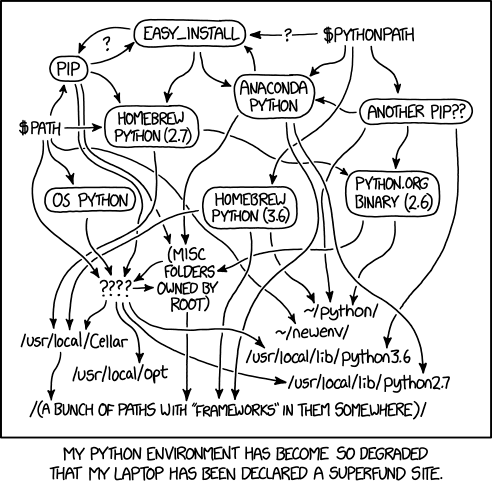
\includegraphics[width=6.83in]{figures/advanced/python-environment}
  \caption{XKCD on Python Environments (from https://xkcd.com/1987/)}
  \label{fig:xkcd}
\end{figure}

\subsection*{How can we access data across languages?}

The most common way to use \texttt{reticulate} is
to do some calculations in Python and then use the results in R
or vice versa.
To show how this works,
let's read our infant HIV data into a Pandas data frame:

\begin{lstlisting}
import pandas
data = pandas.read_csv('results/infant_hiv.csv')
print(data.head())
\end{lstlisting}

\begin{lstlisting}
  country  year  estimate  hi  lo
0     AFG  2009       NaN NaN NaN
1     AFG  2010       NaN NaN NaN
2     AFG  2011       NaN NaN NaN
3     AFG  2012       NaN NaN NaN
4     AFG  2013       NaN NaN NaN
\end{lstlisting}

All of our Python variables are available in our R session as part of the \texttt{py} object,
so we use \texttt{py\$data} to access this data from R:

\begin{lstlisting}
library(reticulate)
head(py$data)
\end{lstlisting}

\begin{lstlisting}
  country year estimate  hi  lo
1     AFG 2009      NaN NaN NaN
2     AFG 2010      NaN NaN NaN
3     AFG 2011      NaN NaN NaN
4     AFG 2012      NaN NaN NaN
5     AFG 2013      NaN NaN NaN
6     AFG 2014      NaN NaN NaN
\end{lstlisting}

\texttt{reticulate} handles type conversions automatically,
though there are a few tricky cases:
for example,
the number \texttt{9} is a float in R,
so if you want it to be an integer in Python,
you have to write it as \texttt{(L}
(where the ``L'' stands for for ``long'').

The good news is that
\texttt{reticulate} translates between Python's 0-based indexing
and the 1-based indexing used by R (and human beings).
Suppose we create a character vector in R:

\begin{lstlisting}
elements = c('hydrogen', 'helium', 'lithium', 'beryllium')
\end{lstlisting}

\noindent
Hydrogen is in position 1 in R:

\begin{lstlisting}
elements[1]
\end{lstlisting}

\begin{lstlisting}
[1] "hydrogen"
\end{lstlisting}

\noindent
but position 0 in Python:

\begin{lstlisting}
print(r.elements[0])
\end{lstlisting}

\begin{lstlisting}
hydrogen
\end{lstlisting}

\noindent
Notice our use of the object \texttt{r} in our Python:
just \texttt{py\$whatever} gives us access to Python objects in R,
\texttt{r.whatever} gives us access to R objects in Python.

\subsection*{How can we call functions across languages?}

We don't have to run Python code,
store values in a variable,
and then access that variable from R:
we can call the Python directly (or vice versa).
For example,
we can use Python's random number generator in R:

\begin{lstlisting}
pyrand <- import("random")
pyrand$gauss(0, 1)
\end{lstlisting}

\begin{lstlisting}
[1] -1.086699
\end{lstlisting}

We can also source Python scripts.
For example,
suppose that \texttt{countries.py} contains:

\begin{lstlisting}
#!/usr/bin/env python

import pandas as pd

def get_countries(filename):
    data = pd.read_csv(filename)
    return data.country.unique()
\end{lstlisting}

\noindent
We can run that script using \texttt{source\_python}:

\begin{lstlisting}
source_python('countries.py')
\end{lstlisting}

This call does not produce any output because all the script did was define a function.
However,
that function and all other top-level variables defined in the script are now available in R:

\begin{lstlisting}
get_countries('results/infant_hiv.csv')
\end{lstlisting}

\begin{lstlisting}
  [1] "AFG" "AGO" "AIA" "ALB" "ARE" "ARG" "ARM" "ATG" "AUS" "AUT"
 [11] "AZE" "BDI" "BEL" "BEN" "BFA" "BGD" "BGR" "BHR" "BHS" "BIH"
 [21] "BLR" "BLZ" "BOL" "BRA" "BRB" "BRN" "BTN" "BWA" "CAF" "CAN"
...and many more rows...
\end{lstlisting}

There is one small pothole in this, though.
When the script is run,
the special Python variable \texttt{\_\_name\_\_} is set to \texttt{'\_\_main\_\_'},
just as it is would be if the script was run directly on the command line.
If the script includes a conditional block to handle command-line arguments,
such as:

\begin{lstlisting}
if __name__ == '__main__':
    input_file, output_files = sys.argv[1], sys.argv[2:]
    main(input_file, output_files)
\end{lstlisting}

\noindent
then that block will be executed,
but will fail because \texttt{sys.argv} won't include anything.

\section{How does object-oriented programming work in R?}\label{advanced-oop}

Programmers spend a great deal of their time trying to create order out of chaos,
and the rest of their time inventing new ways to create more chaos.
Object-oriented programming serves both needs well:
it allows good software designers to create marvels,
and less conscientious or less experienced ones to manufacture horrors.

R has not one,
not two,
but at least three different frameworks for object-oriented programming.
By far the most widely used is called S3
(because it was first introduced with Version~3 of S,
the language from which R is derived).
Unlike the approaches used in Python and similarly pedestrian languages,
S3 does not require its users to define classes.
Instead,
they add \gref{g:attribute}{attributes} to data,
then write specialized versions of \gref{g:generic-function}{generic functions}
to process the data according to those attributes.
Since attributes can be used in other ways as well,
we will start by exploring them.

\subsection*{What are attributes?}

Let's begin by creating a matrix containing the first few hundreds:

\begin{lstlisting}
values <- 100 * 1:9 # creates c(100, 200, ..., 900)
m <- matrix(values, nrow = 3, ncol = 3)
m
\end{lstlisting}

\begin{lstlisting}
     [,1] [,2] [,3]
[1,]  100  400  700
[2,]  200  500  800
[3,]  300  600  900
\end{lstlisting}

Behind the scenes,
R to store our nine values as a vector.
However,
it adds an attribute called \texttt{class} to the vector to identify it as a matrix:

\begin{lstlisting}
class(m)
\end{lstlisting}

\begin{lstlisting}
[1] "matrix"
\end{lstlisting}

\noindent
and another attribute called \texttt{dim} to store its dimensions as a 2-element vector:

\begin{lstlisting}
dim(m)
\end{lstlisting}

\begin{lstlisting}
[1] 3 3
\end{lstlisting}

An object's attributes are simply a set of name-value pairs.
We can find out what attributes are present using \texttt{attributes}
and show or set individual attributes using \texttt{attr}:

\begin{lstlisting}
attr(m, "prospects") <- "dismal"
attributes(m)
\end{lstlisting}

\begin{lstlisting}
$dim
[1] 3 3

$prospects
[1] "dismal"
\end{lstlisting}

What are the type and attributes of a tibble?

\begin{lstlisting}
t <- tribble(
  ~a, ~b,
  1, 2,
  3, 4)
typeof(t)
\end{lstlisting}

\begin{lstlisting}
[1] "list"
\end{lstlisting}

\begin{lstlisting}
attributes(t)
\end{lstlisting}

\begin{lstlisting}
$names
[1] "a" "b"

$row.names
[1] 1 2

$class
[1] "tbl_df"     "tbl"        "data.frame"
\end{lstlisting}

This tells us that a tibble is stored as a list (the first line of output),
and that it has an attribute called \texttt{names} that stores the names of its columns,
another called \texttt{row.names} that stores the names of its rows (a feature we should ignore),
and three classes \texttt{tbl\_df}, \texttt{tbl}, and \texttt{data.frame}.
These classes tell R what functions to search for when we do things like
ask for the length of a tibble (which is the number of rows it contains):

\begin{lstlisting}
length(t)
\end{lstlisting}

\begin{lstlisting}
[1] 2
\end{lstlisting}

\noindent
The order of the classes is important:
when we call \texttt{length(t)},
R looks for a function associated with \texttt{tbl\_df}, \texttt{tbl}, or \texttt{data.frame}
\emph{in that order}.

\subsection*{How are classes represented?}

To show how classes and generic functions work together,
let's customize the way that 2D coordinates are converted to strings.
First,
we create two coordinate vectors:

\begin{lstlisting}
first <- c(0.5, 0.7)
class(first) <- "two_d"
print(first)
\end{lstlisting}

\begin{lstlisting}
[1] 0.5 0.7
attr(,"class")
[1] "two_d"
\end{lstlisting}

\begin{lstlisting}
second <- c(1.3, 3.1)
class(second) <- "two_d"
print(second)
\end{lstlisting}

\begin{lstlisting}
[1] 1.3 3.1
attr(,"class")
[1] "two_d"
\end{lstlisting}

Separately,
we define the behavior of \texttt{toString} for such objects:

\begin{lstlisting}
toString.two_d <- function(obj){
  paste0("<", obj[1], ", ", obj[2], ">")
}
toString(first)
\end{lstlisting}

\begin{lstlisting}
[1] "<0.5, 0.7>"
\end{lstlisting}

\begin{lstlisting}
toString(second)
\end{lstlisting}

\begin{lstlisting}
[1] "<1.3, 3.1>"
\end{lstlisting}

S3's protocol is simple:
given a function \texttt{F} and an object of class \texttt{C},
S3 looks for a function named \texttt{F.C}
(i.e., \texttt{F}, dot, and \texttt{C}).
If it doesn't find one,
it tries the object's next class;
once the object's classes are exhausted,
it uses whatever function the system has defined for the object's base type
(in this case, character vector).
We can trace this process by importing the \texttt{sloop} package
and calling \texttt{s3\_dispatch}:

\begin{lstlisting}
library(sloop)
s3_dispatch(toString(first))
\end{lstlisting}

\begin{lstlisting}
=> toString.two_d
 * toString.default
\end{lstlisting}

\noindent
Compare this with calling \texttt{toString} on a plain old character vector:

\begin{lstlisting}
s3_dispatch(toString(c(7.1, 7.2)))
\end{lstlisting}

\begin{lstlisting}
   toString.double
   toString.numeric
=> toString.default
\end{lstlisting}

The specialized functions associated with a generic function like \texttt{toString}
are called \gref{g:method}{methods}.
Unlike languages that require methods to be defined all together as part of a class,
S3 allows us to add methods when and as we see fit.
But that doesn't mean we should:
minds confined to three dimensions of space and one of time
are simply not capable of comprehending complex class hierarchies.
Instead,
we should always write three functions that work together
to create a class like \texttt{two\_d}:

\begin{itemize}
\item
  A \gref{g:constructor}{constructor} called \texttt{new\_two\_d}
  that creates objects.
\item
  An optional \gref{g:validator}{validator} called \texttt{validate\_two\_d}
  that checks the consistency and correctness of an object's values.
\item
  An optional \gref{g:helper}{helper},
  simply called \texttt{two\_d},
  that most users will call to create and validate objects.
\end{itemize}

The constructor's first argument should always be the base object (in our case, the two-element vector).
It should also have one argument for each attribute the object is to have, if any.
Unlike matrices, our 2D points don't have any extra arguments, so our constructor needs no extra arguments.
Crucially,
the constructor checks the type of its arguments to ensure that the object has at least some chance of being valid:

\begin{lstlisting}
new_two_d <- function(coordinates){
  stopifnot(is.numeric(coordinates))
  class(coordinates) <- "two_d"
  coordinates
}

example <- new_two_d(c(4.4, -2.2))
toString(example)
\end{lstlisting}

\begin{lstlisting}
[1] "<4.4, -2.2>"
\end{lstlisting}

Validators are only needed when checks on data correctness and consistency are expensive.
For example,
if we were to define a class to represent sorted vectors,
checking that elements are in order could take a long time for very long vectors.
To illustrate this,
we will check that we have exactly two coordinates;
in real code,
we would probably include this (inexpensive) check in the constructor:

\begin{lstlisting}
validate_two_d <- function(coordinates) {
  stopifnot(length(coordinates) == 2)
  stopifnot(class(coordinates) == "two_d")
}

validate_two_d(example)    # should succeed silently
validate_two_d(c(1, 3))    # should fail
validate_two_d(c(2, 2, 2)) # should also fail
\end{lstlisting}

\begin{lstlisting}
Error in validate_two_d(c(1, 3)): class(coordinates) == "two_d" is not TRUE
Error in validate_two_d(c(2, 2, 2)): length(coordinates) == 2 is not TRUE
\end{lstlisting}

The third and final function in our trio
provides a user-friendly way to construct objects of our new class.
It should call the constructor and the validator (if one exists),
but should also provide a richer set of defaults,
better error messages,
and so on.
To illustrate this,
we shall allow the user to provide either one argument (which must be a two-element vector)
or two (which must each be numeric):

\begin{lstlisting}
two_d <- function(...){
  args <- list(...)
  if (length(args) == 1) {
    args <- args[[1]]    # extract original value
  }
  else if (length(args) == 2) {
    args <- unlist(args) # convert list to vector
  }
  result <- new_two_d(args)
  validate_two_d(result)
  result
}

here <- two_d(10.1, 11.2)
toString(here)
\end{lstlisting}

\begin{lstlisting}
[1] "<10.1, 11.2>"
\end{lstlisting}

\begin{lstlisting}
there <- two_d(c(15.6, 16.7))
toString(there)
\end{lstlisting}

\begin{lstlisting}
[1] "<15.6, 16.7>"
\end{lstlisting}

\subsection*{How does inheritance work?}

We said above that an object can have more than one class,
and that S3 searches the classes in order when it wants to find a method to call.
Methods can also trigger invocation of other methods explicitly in order to supplement,
rather than replace,
the behavior of other classes.
To show how this works,
we shall look at that classic of object-oriented design: shapes.
(The safe kind,
of course,
not those whose non-Euclidean angles have placed such intolerable stress
on the minds of so many of our colleagues over the years.)

We start by defining a \texttt{polygon} class:

\begin{lstlisting}
new_polygon <- function(coords, name) {
  points <- map(coords, two_d)
  class(points) <- "polygon"
  attr(points, "name") <- name
  points
}

toString.polygon <- function(poly) {
  paste0(attr(poly, "name"), ": ", paste0(map(poly, toString), collapse = ", "))
}

right <- new_polygon(list(c(0, 0), c(1, 0), c(0, 1)), "triangle")
toString(right)
\end{lstlisting}

\begin{lstlisting}
[1] "triangle: <0, 0>, <1, 0>, <0, 1>"
\end{lstlisting}

\noindent
Next we add colored shapes:

\begin{lstlisting}
new_colored_polygon <- function(coords, name, color) {
  object <- new_polygon(coords, name)
  attr(object, "color") <- color
  class(object) <- c("colored_polygon", class(object))
  object
}

pinkish <- new_colored_polygon(list(c(0, 0), c(1, 0), c(1, 1)), "triangle", "roseate")
class(pinkish)
\end{lstlisting}

\begin{lstlisting}
[1] "colored_polygon" "polygon"        
\end{lstlisting}

\begin{lstlisting}
toString(pinkish)
\end{lstlisting}

\begin{lstlisting}
[1] "triangle: <0, 0>, <1, 0>, <1, 1>"
\end{lstlisting}

So far so good:
since we have not defined a method to handle colored polygons specifically,
we get the behavior for a regular polygon.
Let's add another method that supplements the behavior of the existing method:

\begin{lstlisting}
toString.colored_polygon <- function(poly) {
  paste0(toString.polygon(poly), "+ color = ", attr(poly, "color"))
}

toString(pinkish)
\end{lstlisting}

\begin{lstlisting}
[1] "triangle: <0, 0>, <1, 0>, <1, 1>+ color = roseate"
\end{lstlisting}

In practice,
we will almost always place all of the methods associated with a class
in the same file as its constructor, validator, and helper.

\section{How can we work with relational databases in R?}\label{advanced-db}

Data frames and database tables go together
as naturally as dark chocolate and the tears of our vanquished enemies.
As in Python and other languages,
there is a standard interface for connecting to and querying relational databases;
each database is then supported by a package that implements that interface.
This doesn't completely hide their differences---we must still worry about
the quirks of various SQL dialects---but it does keep the R side of things simple.

This tutorial uses the SQLite database and the \texttt{RSQLite} interface package.
The former is included with the latter,
so \texttt{install.packages("RSQLite")} will give you everything you need.
We assume that you already speak enough SQL to get yourself into trouble;
if you do not,
the \href{https://swcarpentry.github.io/sql-novice-survey/}{Software Carpentry tutorial}
is a good place to start.

\subsection*{How can we get data from a database?}

Suppose we have a small database in \texttt{example.db}
containing survey data salvaged from
a series of doomed expeditions to the Antarctic in the 1920s and 1930s.
The database contains four tables:

\noindent
\textbf{Person}: people who took readings.

\begin{longtable}[]{lll}
person\_id & personal & family\\
dyer & William & Dyer\\
pb & Frank & Pabodie\\
lake & Anderson & Lake\\
roe & Valentina & Roerich\\
danforth & Frank & Danforth\\
\end{longtable}

\noindent
\textbf{Site}: locations where readings were taken.

\begin{longtable}[]{lll}
site\_id & lat & long\\
DR-1 & -49.85 & -128.57\\
DR-3 & -47.15 & -126.72\\
MSK-4 & -48.87 & -123.4\\
\end{longtable}

\noindent
\textbf{Visited}: when readings were taken at specific sites.
(\texttt{-null-} is used to show missing values.)

\begin{longtable}[]{lll}
visit\_id & site\_id & dated\\
619 & DR-1 & 1927-02-08\\
622 & DR-1 & 1927-02-10\\
734 & DR-3 & 1930-01-07\\
735 & DR-3 & 1930-01-12\\
751 & DR-3 & 1930-02-26\\
752 & DR-3 & -null-\\
837 & MSK-4 & 1932-01-14\\
844 & DR-1 & 1932-03-22\\
\end{longtable}

\noindent
\textbf{Measurements}: the actual readings.

\begin{longtable}[]{llll}
visit\_id & visitor & quantity & reading\\
619 & dyer & rad & 9.82\\
619 & dyer & sal & 0.13\\
622 & dyer & rad & 7.8\\
622 & dyer & sal & 0.09\\
734 & pb & rad & 8.41\\
734 & lake & sal & 0.05\\
734 & pb & temp & -21.5\\
735 & pb & rad & 7.22\\
735 & -null- & sal & 0.06\\
735 & -null- & temp & -26.0\\
751 & pb & rad & 4.35\\
751 & pb & temp & -18.5\\
751 & lake & sal & 0.1\\
752 & lake & rad & 2.19\\
752 & lake & sal & 0.09\\
752 & lake & temp & -16.0\\
752 & roe & sal & 41.6\\
837 & lake & rad & 1.46\\
837 & lake & sal & 0.21\\
837 & roe & sal & 22.5\\
844 & roe & rad & 11.25\\
\end{longtable}

Let's get the people into a data frame:

\begin{lstlisting}
library(DBI)
db <- dbConnect(RSQLite::SQLite(), here::here("data", "example.db"))
dbGetQuery(db, "select * from Person;")
\end{lstlisting}

\begin{lstlisting}
  person_id personal_name family_name
1      dyer       William        Dyer
2        pb         Frank     Pabodie
3      lake      Anderson        Lake
4       roe     Valentina     Roerich
5  danforth         Frank    Danforth
\end{lstlisting}

That seems simple enough:
the database connection is the first argument to \texttt{dbGetQuery},
the query itself is the second,
and the result is a tibble whose column names correspond to the names of the fields in the database table.
What if we want to parameterize our query?
Inside the text of the query,
we use \texttt{:name} as a placeholder for a query parameter,
then pass a list of name-value pairs to specify what we actually want:

\begin{lstlisting}
dbGetQuery(db,
           "select * from Measurements where quantity = :desired",
           params = list(desired = "rad"))
\end{lstlisting}

\begin{lstlisting}
  visit_id person_id quantity reading
1      619      dyer      rad    9.82
2      622      dyer      rad    7.80
3      734        pb      rad    8.41
4      735        pb      rad    7.22
5      751        pb      rad    4.35
6      752      lake      rad    2.19
7      837      lake      rad    1.46
8      844       roe      rad   11.25
\end{lstlisting}

\noindent
Do \emph{not} use \texttt{glue} or some other kind of string interpolation
to construct database queries,
as this can leave you open to
\href{https://en.wikipedia.org/wiki/SQL_injection}{SQL injection attacks}
and other forms of digital damnation.

If you expect a large set of results,
it's best to page through them:

\begin{lstlisting}
results <- dbSendQuery(db, "select * from Measurements limit 15;")
while (!dbHasCompleted(results)) {
  chunk <- dbFetch(results, n = 3) # artificially low for tutorial purposes
  print(chunk)
}
dbClearResult(results)
\end{lstlisting}

\begin{lstlisting}
  visit_id person_id quantity reading
1      619      dyer      rad    9.82
2      619      dyer      sal    0.13
3      622      dyer      rad    7.80
  visit_id person_id quantity reading
1      622      dyer      sal    0.09
2      734        pb      rad    8.41
3      734      lake      sal    0.05
  visit_id person_id quantity reading
1      734        pb     temp  -21.50
2      735        pb      rad    7.22
3      735      <NA>      sal    0.06
  visit_id person_id quantity reading
1      735      <NA>     temp  -26.00
2      751        pb      rad    4.35
3      751        pb     temp  -18.50
\end{lstlisting}

\begin{lstlisting}
Warning in result_fetch(res@ptr, n = n): Column `reading`: mixed type,
first seen values of type real, coercing other values of type string
\end{lstlisting}

\begin{lstlisting}
  visit_id person_id quantity reading
1      751      lake      sal    0.00
2      752      lake      rad    2.19
3      752      lake      sal    0.09
\end{lstlisting}

\subsection*{How can we populate databases with R?}

Data scientists spend most of their time reading data,
but someone has to create it.
\texttt{RSQLite} makes it easy to map a data frame directly to a database table;
to show how it works,
we will create an in-memory database:

\begin{lstlisting}
colors <- tribble(
  ~name, ~red, ~green, ~blue,
  'black', 0, 0, 0,
  'yellow', 255, 255, 0,
  'aqua', 0, 255, 255,
  'fuchsia', 255, 0, 0
)
db <- dbConnect(RSQLite::SQLite(), ':memory:')
dbWriteTable(db, "colors", colors)
\end{lstlisting}

Let's see what the combination of R and SQLite has done with our data and the types thereof:

\begin{lstlisting}
dbGetQuery(db, "select * from colors;")
\end{lstlisting}

\begin{lstlisting}
     name red green blue
1   black   0     0    0
2  yellow 255   255    0
3    aqua   0   255  255
4 fuchsia 255     0    0
\end{lstlisting}

Good: the types have been guessed correctly.
But what about dates?

\begin{lstlisting}
appointments <- tribble(
  ~who, ~when,
  'Dyer', '1927-03-01',
  'Peabody', '1927-05-05'
) %>% mutate(when = lubridate::as_date(when))
dbWriteTable(db, "appointments", appointments)
dbGetQuery(db, "select * from appointments;")
\end{lstlisting}

\begin{lstlisting}
      who   when
1    Dyer -15647
2 Peabody -15582
\end{lstlisting}

What fresh hell is this?
After considerable trial and error,
we discover that our dates have been returned to us as
the number of days since January 1, 1970:

\begin{lstlisting}
dbExecute(db,
           "insert into appointments values('Testing', :the_date);",
           params = list(the_date = lubridate::as_date('1971-01-01')))
dbGetQuery(db, "select * from appointments where who = 'Testing';")
\end{lstlisting}

\begin{lstlisting}
[1] 1
      who when
1 Testing  365
\end{lstlisting}

\noindent
There is no point screaming:
those who might pity you cannot hear,
and those who can hear know nothing of pity.

\section{How can we write web applications in R?}

R has this awesome gnarly web programming framework called Shiny.
It uses \st{sympathetic magic} \st{quantum entanglement} reactive variables
to update the application's interface when data changes.
You should, like, totally check it out.

\section{Key Points}

\begin{itemize}
\item
  The \texttt{reticulate} library allows R programs to access data in Python programs and vice versa.
\item
  Use \texttt{py.whatever} to access a top-level Python variable from R.
\item
  Use \texttt{r.whatever} to access a top-level R definition from Python.
\item
  R is always indexed from 1 (even in Python) and Python is always indexed from 0 (even in R).
\item
  Numbers in R are floating point by default, so use a trailing `L' to force a value to be an integer.
\item
  A Python script run from an R session believes it is the main script, i.e., \texttt{\_\_name\_\_} is \texttt{'\_\_main\_\_'} inside the Python script.
\item
  S3 is the most commonly used object-oriented programming system in R.
\item
  Every object can store metadata about itself in attributes, which are set and queried with \texttt{attr}.
\item
  The \texttt{dim} attribute stores the dimensions of a matrix (which is physically stored as a vector).
\item
  The \texttt{class} attribute of an object defines its class or classes (it may have several character entries).
\item
  When \texttt{F(X,\ ...)} is called, and \texttt{X} has class \texttt{C}, R looks for a function called \texttt{F.C} (the \texttt{.} is just a naming convention).
\item
  If an object has multiple classes in its \texttt{class} attribute, R looks for a corresponding method for each in turn.
\item
  Every user defined class \texttt{C} should have functions \texttt{new\_C} (to create it), \texttt{validate\_C} (to validate its integrity), and \texttt{C} (to create and validate).
\item
  Use the \texttt{DBI} package to work with relational databases.
\item
  Use \texttt{DBI::dbConnect(...)} with database-specific parameters to connect to a specific database.
\item
  Use \texttt{dbGetQuery(connection,\ "query")} to send an SQL query string to a database and get a data frame of results.
\item
  Parameterize queries using \texttt{:name} as a placeholder in the query and \texttt{params~=~list(name~=~value)} as a third parameter to \texttt{dbGetQuery} to specify actual values.
\item
  Use \texttt{dbFetch} in a \texttt{while} loop to page results.
\item
  Use \texttt{dbWriteTable} to write an entire data frame to a table, and \texttt{dbExecute} to execute a single insertion statement.
\item
  Shiny is cool.
\end{itemize}

\section{Exercises}

\begin{enumerate}

\item
  Create a function in Python that returns a list of lists,
  where the elements of each sublist are of different types:

\begin{lstlisting}
def listOfLists():
    return [['a', 1], [True, ('a', 'tuple')]]
\end{lstlisting}

  \noindent
  Call this function from R.
  What types of data are returned?

\item
  Define a class in Python and create an instance of it:

\begin{lstlisting}
class Thing:
    def method():
        return 'method of thing'

myThing = Thing()
\end{lstlisting}

  \noindent
  How does \texttt{myThing} appear in an R program?
  How can we call \texttt{myThing.method}?

\item
  Create a polygon (colored or uncolored) using the code from Section~\ref{advanced-oop}
  and then inspect it in Python.
  What kind of thing does Python see?
  (How) can we call the right methods for polygons from Python?

\item
  This question uses the \texttt{example.db} database from Section~\ref{advanced-db}.
  \begin{enumerate}
  \item
    Write a SQL query to join the \texttt{Site} and \texttt{Visited} tables
    using the \texttt{site\_id} key from each,
    and use \texttt{RSQLite} to send that query to the database.
  \item
    Write one small SQL query to get all the data from the \texttt{Site} table
    and a second query to get all the data from the \texttt{Visited} table,
    then use \texttt{dplyr::join} to join the tables.
  \end{enumerate}
  Which approach do you find easier to write?
  Which is easier to read?

\end{enumerate}
